
% This LaTeX was auto-generated from MATLAB code.
% To make changes, update the MATLAB code and republish this document.
\documentclass[12pt]{article}
\usepackage{fullpage}
\usepackage[top=10mm, bottom=37mm, left=10mm, right=10mm]{geometry}
\usepackage{amsmath,amsthm,amssymb}
\usepackage{lastpage}
\usepackage{enumerate}
\usepackage{fancyhdr}
\usepackage{xcolor}
\usepackage{graphicx}
\usepackage{listings}
\usepackage{hyperref}
\usepackage{answers}
\usepackage{setspace}
\usepackage{enumitem}
\usepackage{multicol}
\usepackage{mathrsfs}
\usepackage{algorithmic}
\usepackage{stmaryrd}
\usepackage[ruled,linesnumbered,vlined]{algorithm2e}
\usepackage{tikz}
\usetikzlibrary{automata, positioning}

\hypersetup{%
	colorlinks=true,
	linkcolor=blue,
	linkbordercolor={0 0 1}
}

\lstdefinestyle{Python}{
	language        = Python,
	frame           = lines, 
	basicstyle      = \footnotesize,
	keywordstyle    = \color{blue},
	stringstyle     = \color{green},
	commentstyle    = \color{red}\ttfamily
}

\setlength{\parindent}{0.0in}
\setlength{\parskip}{0.05in}

\newcommand\course{\textbf{EE 456}}   
\newcommand\name{Aishwarye Omer}     

\pagestyle{fancyplain}
\headheight 35pt
\lhead{\name\\\course{}}
\chead{\textbf{\Large Homework - 13}}
\rhead{\today}
\lfoot{}
\cfoot{}
\rfoot{\small\thepage}
\headsep 1.5em

\newlength\myindent
\setlength\myindent{2em}
\newcommand\bindent{%
	\begingroup
	\setlength{\itemindent}{\myindent}
	\addtolength{\algorithmicindent}{\myindent}
}
\newcommand\eindent{\endgroup}

\newenvironment{solution}[1][Solution]{\begin{trivlist}
		\item[\hskip \labelsep {\bfseries #1}]}{\end{trivlist}}



\definecolor{lightgray}{gray}{0.5}
\setlength{\parindent}{0pt}

\begin{document}
\textbf{Question:} Competitive netoworks 2
\BlankLine
\textbf{Solution:} 
Following is the code  and result of the network:
\BlankLine
\BlankLine
  \begin{verbatim}
	z1 = 0.2;
	z2 = 0.2;
	z3 = 0.2;
	z4 = 0.2;
	z5 = 0.2;
	z6 = 0.2;
	
	z7 = 0.3;
	z8 = 0.3;
	z9 = 0.3;
	z10 = 0.3;
	z11 = 0.3;
	z12 = 0.3;
	
	c1 = 0.7;
	c2 = -0.3;
	
	z1_new = round(0.7 * (0.2 + 0.2 + 0.2) - 0.3 * (0.2 + 0.2), 2);
	
	z2_new = round(0.7 * (0.2 + 0.2 + 0.2 + 0.2) - 0.3 * (0.2 + 0.2), 2);
	
	z3_new = round(0.7 * (0.2 + 0.2 + 0.2 + 0.2 + 0.2) - 0.3 * (0.2 + 0.3), 2);
	
	z4_new = round(0.7 * (0.2 + 0.2 + 0.2 + 0.2 + 0.2) - 0.3 * (0.2 + 0.3 + 0.3) , 2);
	
	z5_new = round(0.7 * (0.2 + 0.2 + 0.2 + 0.2 + 0.3) - 0.3 * (0.2 + 0.2 + 0.3 + 0.3), 2);
	
	z6_new = round(0.7 * (0.2 + 0.2 + 0.2 + 0.3 + 0.3) - 0.3 * (0.2 + 0.2 + 0.3 + 0.3), 2);
	
	z7_new = round(0.7 * (0.2 + 0.2 + 0.3 + 0.3 + 0.3) - 0.3 * (0.2 + 0.2 + 0.3 + 0.3), 2);
	
	z8_new = round(0.7 * (0.2 + 0.3 + 0.3 + 0.3 + 0.3) - 0.3 * (0.2 + 0.2 + 0.3 + 0.3), 2);
	
	z9_new = round(0.7 * (0.3 + 0.3 + 0.3 + 0.3 + 0.3) - 0.3 * (0.2 + 0.2 + 0.3 + 0.2), 2);
	
	z10_new = round(0.7 * (0.3 + 0.3 + 0.3 + 0.3 + 0.3) - 0.3 * (0.2 + 0.3 + 0.2 + 0.2), 2);
	
	z11_new = round(0.7 * (0.3 + 0.3 + 0.3 + 0.3 + 0.2) - 0.3 * (0.3 + 0.3 + 0.2 + 0.2), 2);
	
	z12_new = round(0.7 * (0.3 + 0.3 + 0.3 + 0.2 + 0.2) - 0.3 * (0.3 + 0.3 + 0.2 + 0.2), 2);
	
	
	fprintf('z1 new = %f\t\n', z1_new );
	fprintf('z2 new = %f\t\n', z2_new );
	fprintf('z3 new = %f\t\n', z3_new );
	fprintf('z4 new = %f\t\n', z4_new );
	fprintf('z5 new = %f\t\n', z5_new );
	fprintf('z6 new = %f\t\n', z6_new );
	fprintf('z7 new = %f\t\n', z7_new );
	fprintf('z8 new = %f\t\n', z8_new );
	fprintf('z9 new = %f\t\n', z9_new );
	fprintf('z10 new = %f\t\n', z10_new );
	fprintf('z11 new = %f\t\n', z11_new );
	fprintf('z12 new = %f\t\n\n\n', z12_new );
	
	Z_old = [z1 z2 z3 z4 z5 z6 z7 z8 z9 z10 z11 z12];
	
	high_old = max(Z_old);
	low_old = min(Z_old);
	amplitude_old = high_old - low_old;
	
	Z_new = [z1_new z2_new z3_new z4_new z5_new z6_new z7_new z8_new z9_new z10_new z11_new z12_new];
	
	high_new = max(Z_new);
	low_new = min(Z_new);
	amplitude_new = high_new - low_new;
	
	fprintf('Amplitude old = %f\t\n\n', amplitude_old );
	fprintf('Amplitude new = %f\t\n', amplitude_new );
	
	%plot(Z_old,'Linewidth',4);
	%plot(Z_new,'Linewidth',4);
\end{verbatim}

\color{lightgray} \begin{verbatim}z1 new = 0.300000	
	z2 new = 0.440000	
	z3 new = 0.550000	
	z4 new = 0.460000	
	z5 new = 0.470000	
	z6 new = 0.540000	
	z7 new = 0.610000	
	z8 new = 0.680000	
	z9 new = 0.780000	
	z10 new = 0.780000	
	z11 new = 0.680000	
	z12 new = 0.610000	
	
	
	Amplitude old = 0.100000	
	
	Amplitude new = 0.480000	
\end{verbatim} 

\begin{figure}[h]
	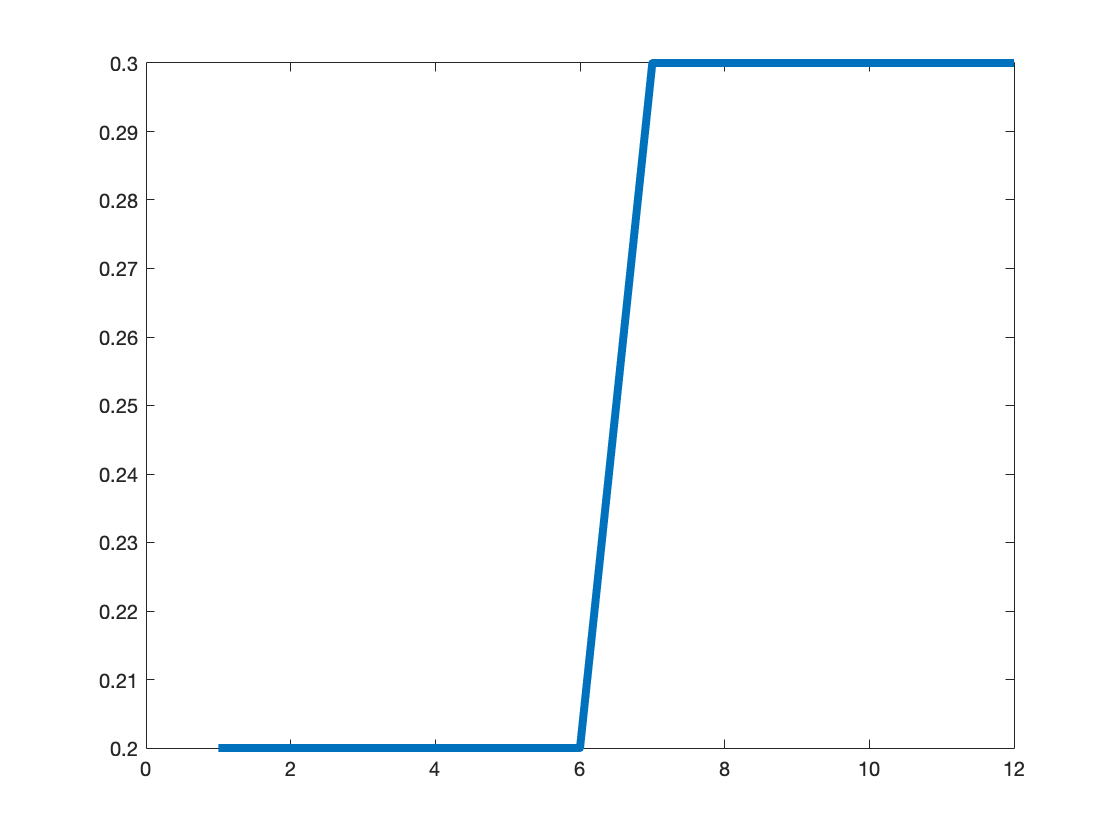
\includegraphics[width=16cm]{Z_old.png}
\end{figure}

\begin{figure}
	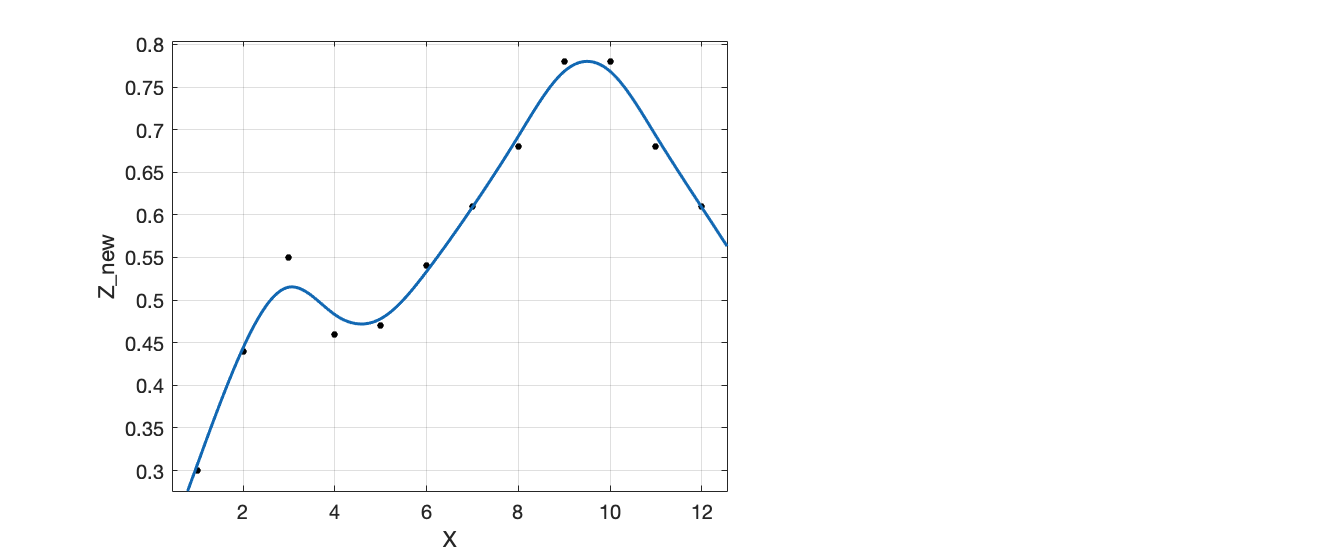
\includegraphics[width=30cm]{Z_new.png}
\end{figure}

\begin{figure}
	\caption{Impulse response}
	\centering
	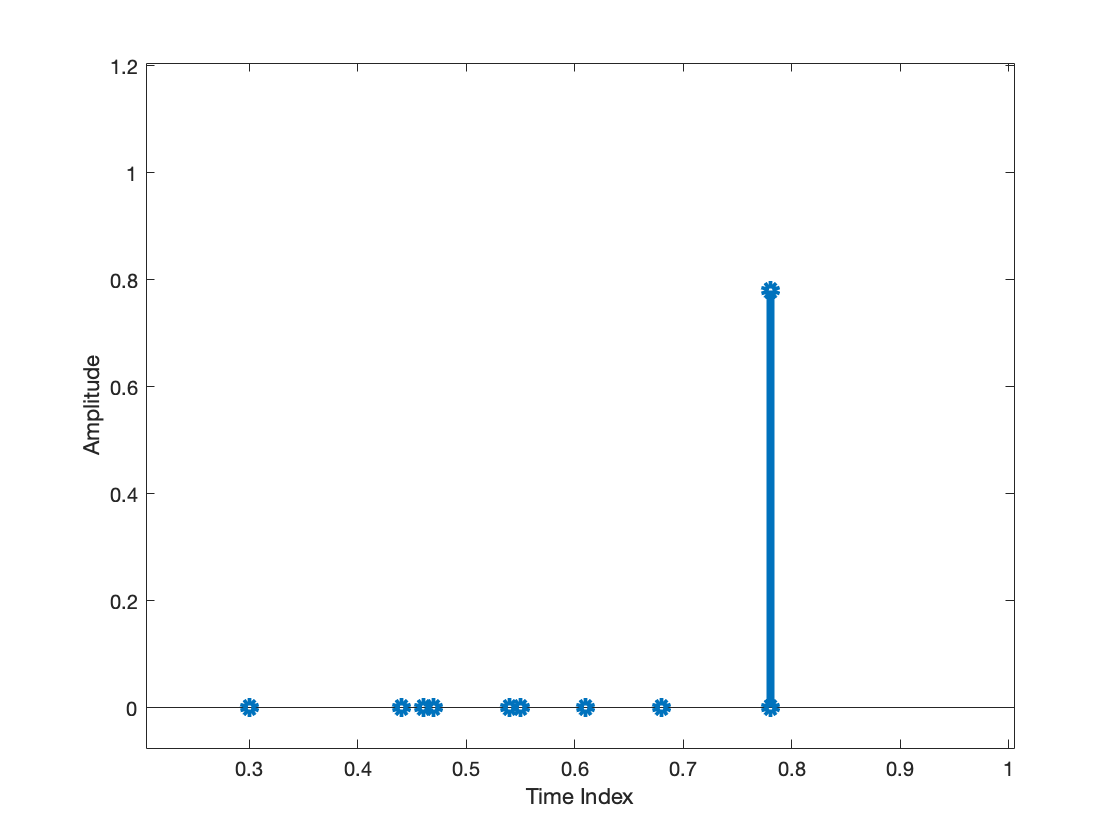
\includegraphics[width=16cm]{impulse.png}

\end{figure}



\end{document}

